\documentclass{article}
\usepackage[backend=biber,citestyle=ieee]{biblatex}
\usepackage[english]{babel}
%\usepackage[swedish]{babel}
\usepackage{graphicx}
\usepackage{csquotes}
\usepackage{float}
\usepackage{subcaption}
\usepackage{url}
\usepackage{float}
\usepackage{siunitx}
\usepackage{datetime}
\usepackage[title]{appendix}
\usepackage[font={small},margin={1cm}]{caption}
\usepackage{titlesec}
\usepackage{enumitem}
\usepackage{amsmath}
\usepackage{fancyhdr}   %page header
\usepackage[margin=1in]{geometry}
\setcounter{secnumdepth}{0}
\pagestyle{fancy}
\fancyhf{}

\cfoot{Page \thepage}

\usepackage[parfill]{parskip} %Line skip between paragraphs instead of indent

\usepackage{xcolor}
\usepackage{listings}   %code section 
\usepackage[hidelinks]{hyperref}



\newcommand{\getauthor}{Eric Johansson (erjo2002@student.miun.se)\\Can Kupeli (caku2002@student.miun.se) \\Samuel Greenberg (sagr1908@student.miun.se)} %Author
\newcommand{\gettitle}{Laboration 2 \\Monte Carlo Simulations} %Title
\newcommand{\getcourse}{(MA069G, Mathematical Modelling 6hp)} %Course
\newcommand{\getsupervisor}{Cornelia Schiebold\\Magnus Eriksson\\Suprokash Hazra}


\begin{document}
\begin{titlepage}
	\begin{center}
		\vspace*{1cm}

		
\includegraphics[width=0.8\textwidth]{imgs/msu.png}\\[0.5cm]
		\Large
		Institution of Information Systems and -Technology (IST)\\[1cm]
		\Huge
		\rule{\textwidth}{1px}
		\textbf{\gettitle}
		\rule[0.5cm]{\textwidth}{1px}

		\large
		\getcourse{}
		\vspace{1cm}

		\Large
		\textbf{\getauthor}\\

		\vfill


		\vspace{0.8cm}

		\small
		\today \\
		\Large
		\textbf{Supervisor:}\\
		\getsupervisor{}

	\end{center}
\end{titlepage}
\tableofcontents
\newpage
\lhead{Laboration 2}
\rhead{Eric, Can, Samuel}


\section{Question 1}
\subsection{(a)}
\begin{figure}[h]
    \begin{subfigure}[h]{0.4\linewidth}
        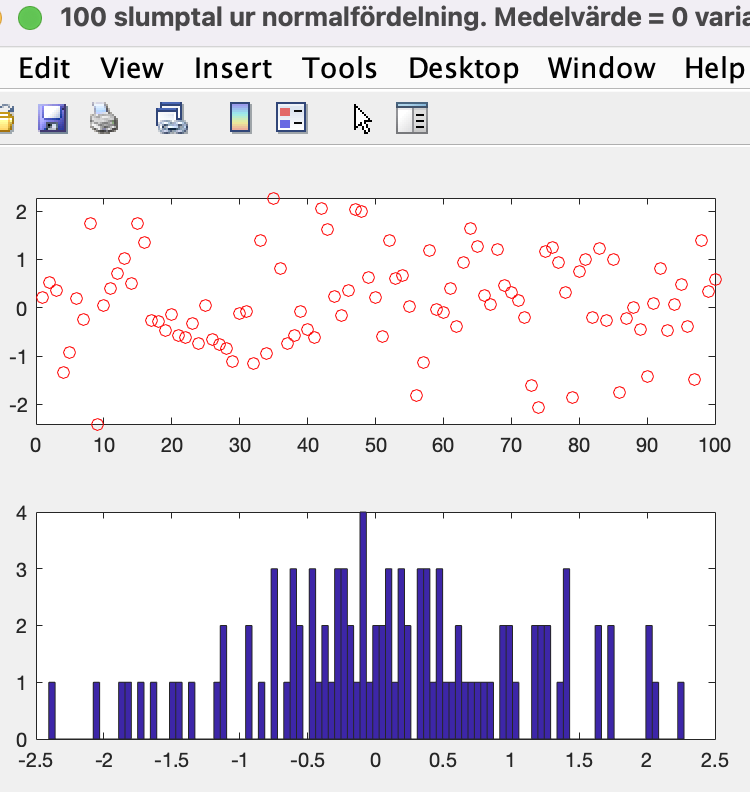
\includegraphics[width=\linewidth]{./imgs/q1a_100.png}
        \caption{100 Randomly generated numbers}
    \end{subfigure}
    \hfill
    \begin{subfigure}[h]{0.4\linewidth}
        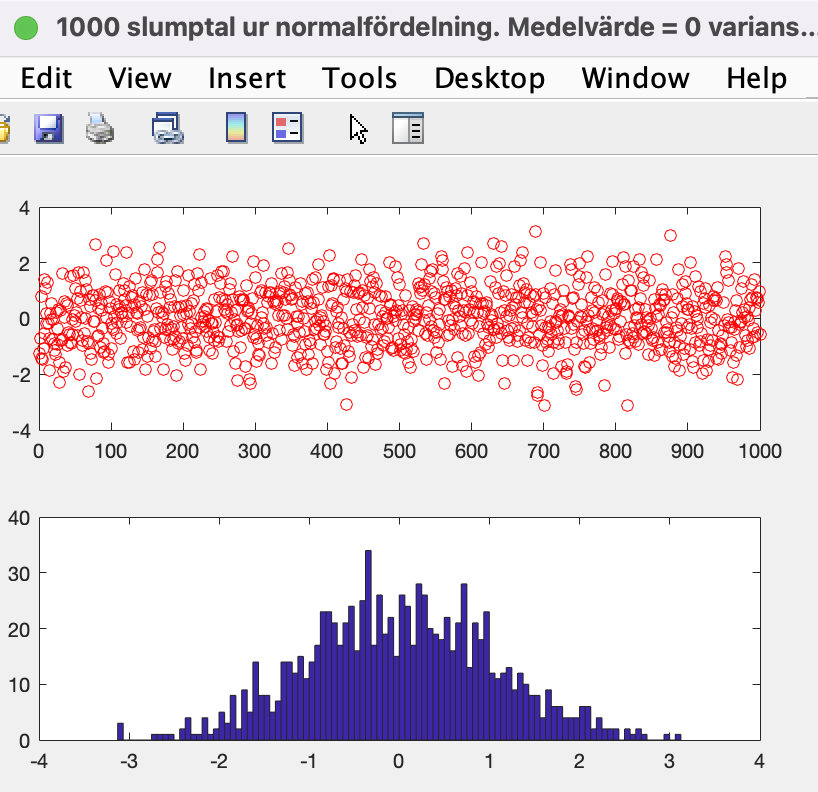
\includegraphics[width=\linewidth]{./imgs/q1a_1000.png}
        \caption{1000 Randomly generated numbers}
    \end{subfigure}
\end{figure}
\begin{figure}[h]
    \begin{subfigure}[h]{0.4\linewidth}
        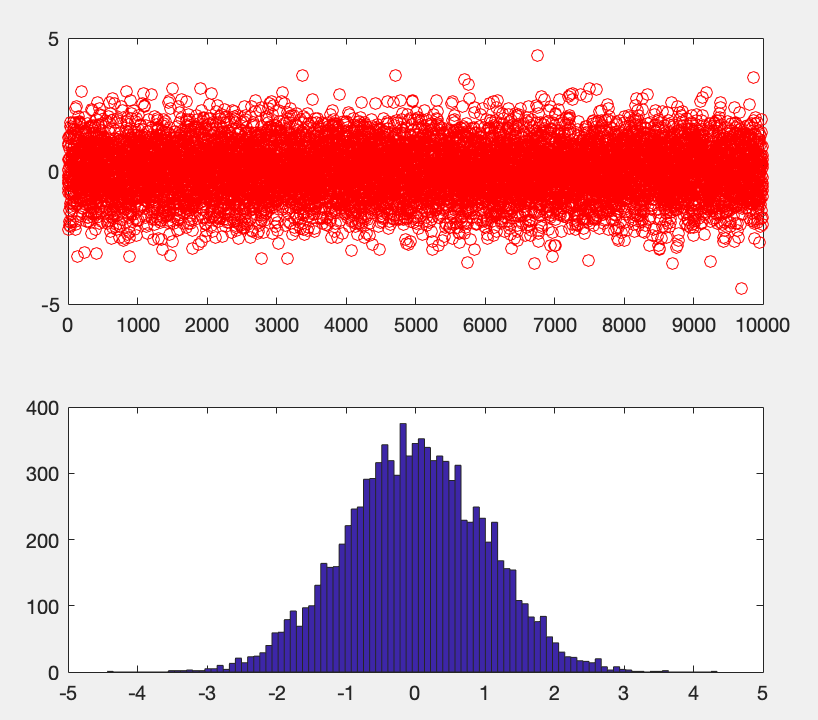
\includegraphics[width=\linewidth]{./imgs/q1a_10000.png}
        \caption{10000 Randomly generated numbers}
    \end{subfigure}
    \hfill
    \begin{subfigure}[h]{0.4\linewidth}
        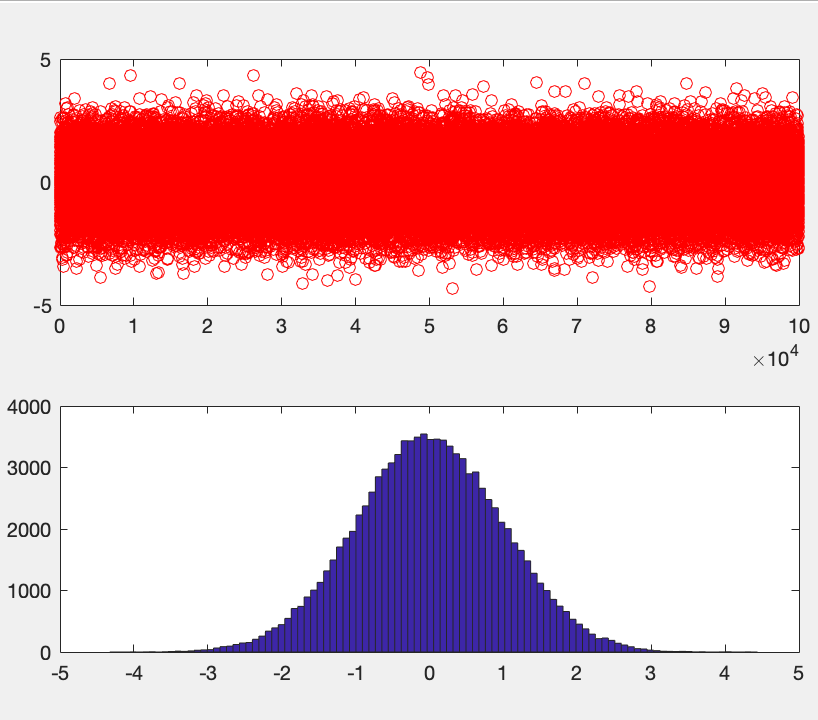
\includegraphics[width=\linewidth]{./imgs/q1a_100000.png}
        \caption{100000 Randomly generated numbers}
    \end{subfigure}
\end{figure}

\begin{figure}[H]
    \begin{subfigure}[h]{0.4\linewidth}
        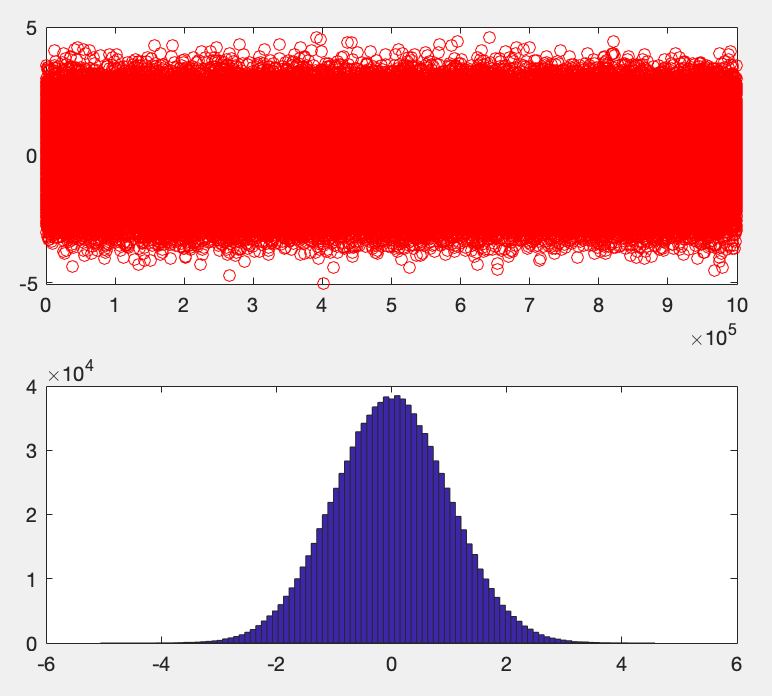
\includegraphics[width=\linewidth]{./imgs/q1a_1000000.png}
        \caption{10000 Randomly generated numbers}
    \end{subfigure}
    \hfill
    \begin{subfigure}[h]{0.4\linewidth}
        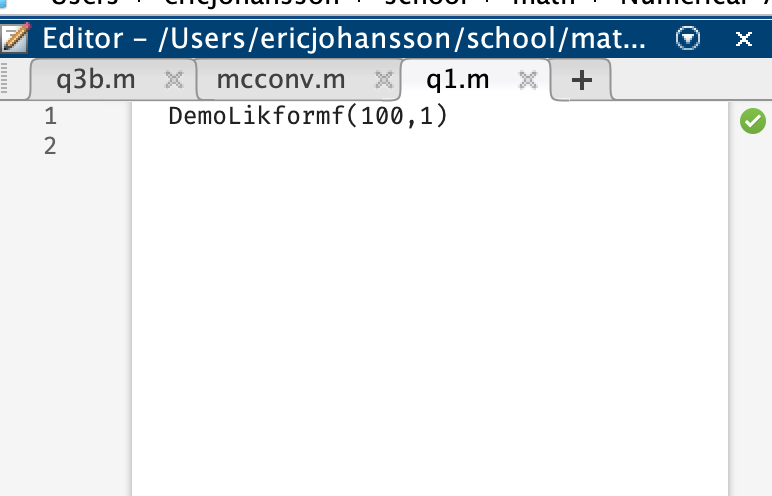
\includegraphics[width=\linewidth]{./imgs/q1_code.png}
        \caption{Code for question 1}
    \end{subfigure}
\end{figure}
As \( N \) icreases the distubution becomes more alike a Normal distribution.


\subsection{(b)}
\begin{figure}[H]
    \begin{subfigure}[h]{0.4\linewidth}
        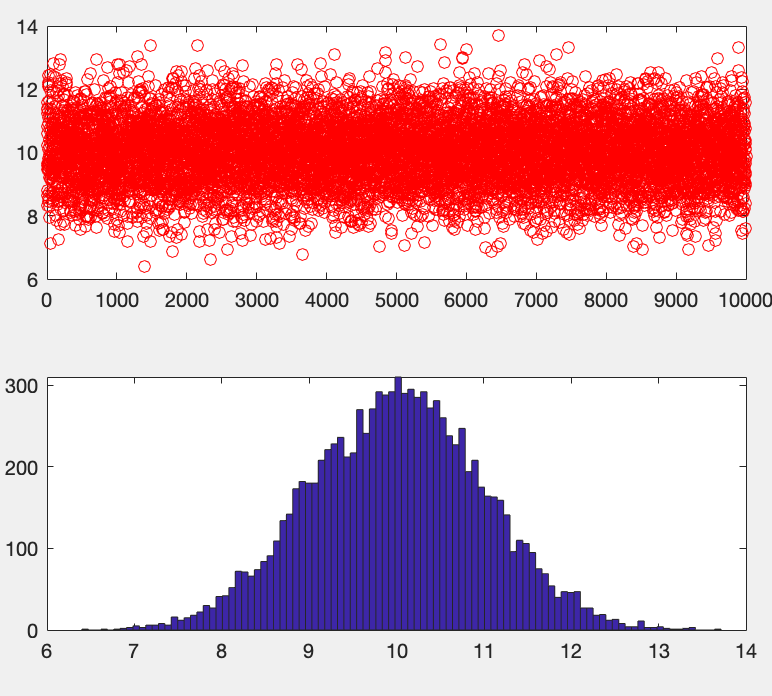
\includegraphics[width=\linewidth]{./imgs/q1b_10.png}
        \caption{\( \mu = \) 10}
    \end{subfigure}
    \hfill
    \begin{subfigure}[h]{0.4\linewidth}
        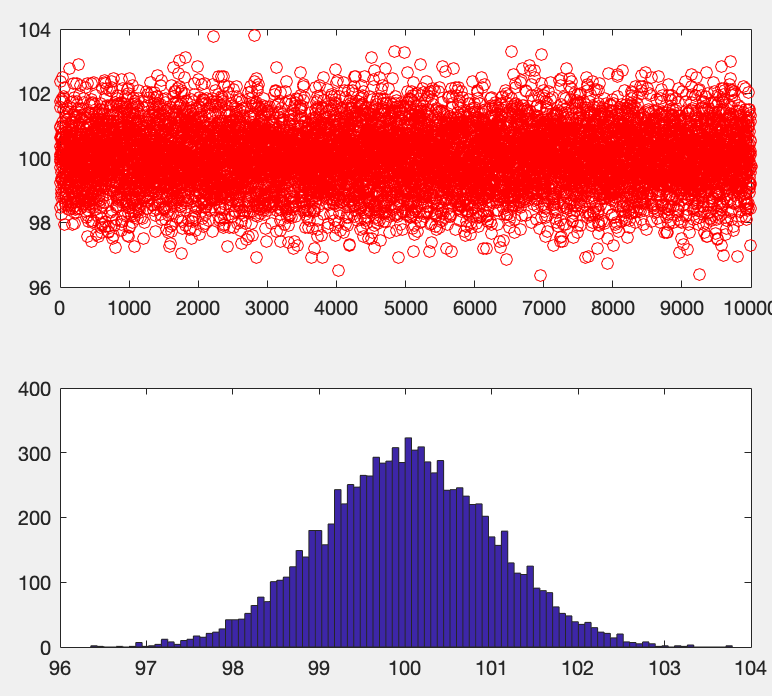
\includegraphics[width=\linewidth]{./imgs/q1b_100.png}
        \caption{\( \mu = \) 100}
    \end{subfigure}
\end{figure}
We can see that the distribution is about the same and the main difference is that they are centered
around different values.

\subsection{(c)}
\begin{figure}[H]
    \begin{subfigure}[h]{0.33\linewidth}
        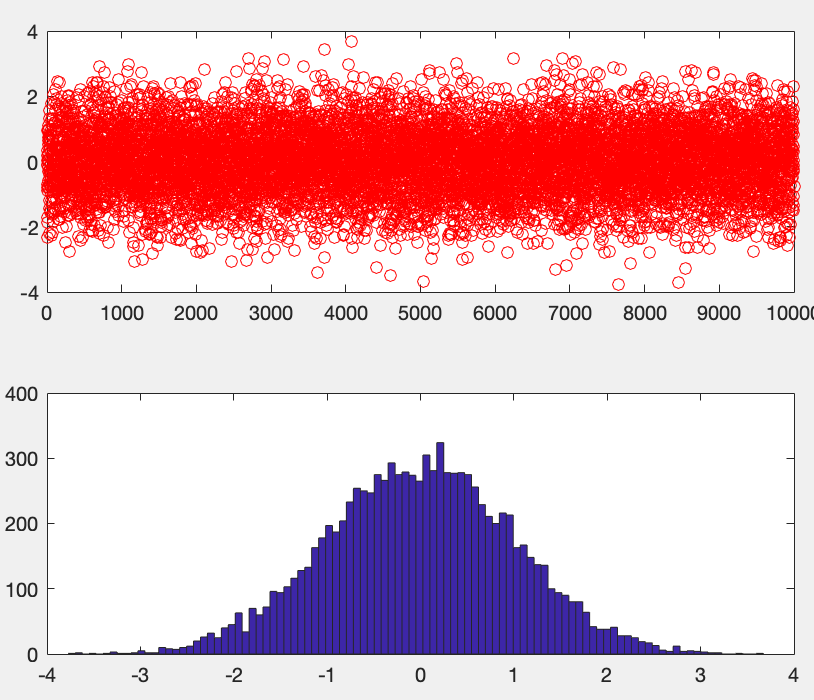
\includegraphics[width=\linewidth]{imgs/q1c_1.png}
        \caption{\( \sigma^2 =1 \)}
    \end{subfigure}
    \begin{subfigure}[h]{0.33\linewidth}
        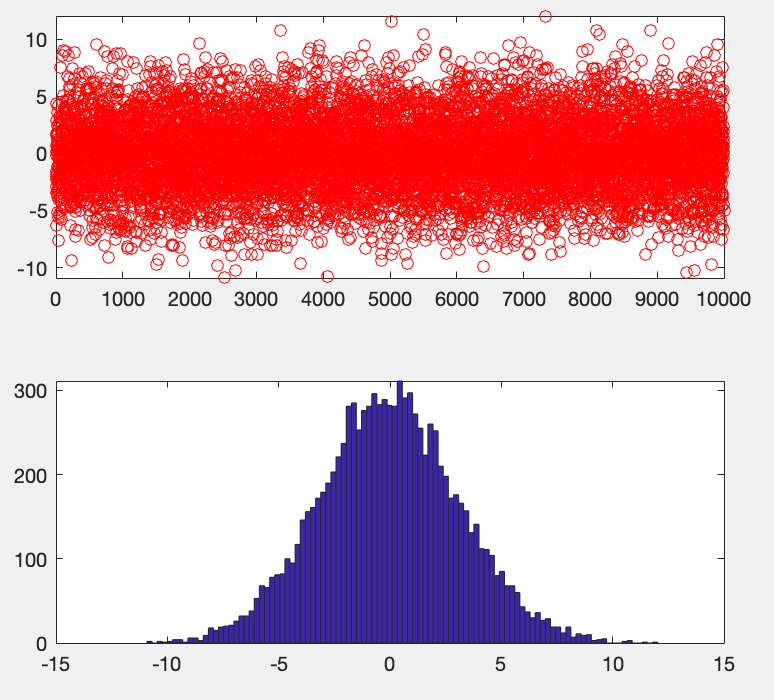
\includegraphics[width=\linewidth]{imgs/q1c_10.png}
        \caption{\( \sigma^2 = 10\)}
    \end{subfigure}
    \begin{subfigure}[h]{0.33\linewidth}
        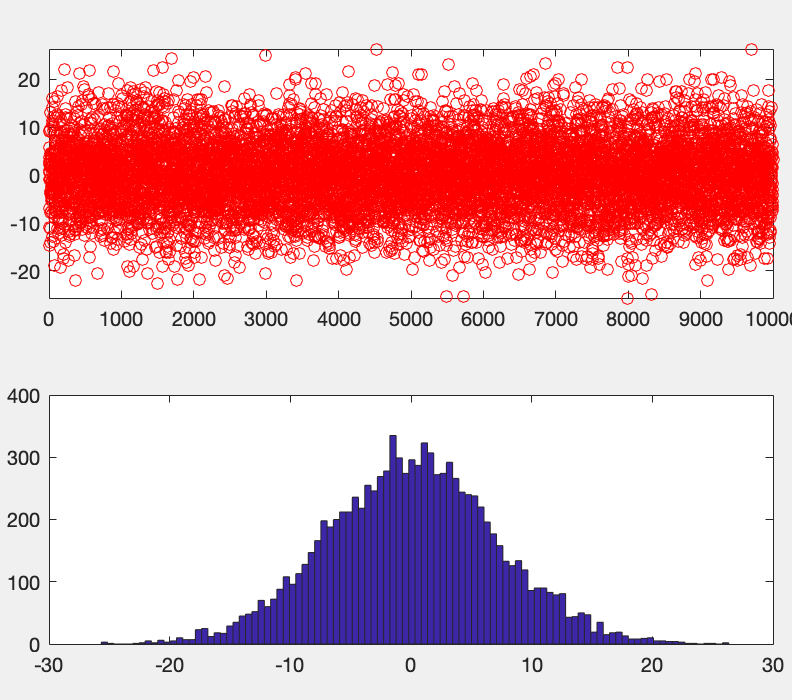
\includegraphics[width=\linewidth]{imgs/q1c_50.png}
        \caption{\( \sigma^2 = 50\)}
    \end{subfigure}
\end{figure}
Once again the form of the distribution is mostly the same, however we can see now that the values
extend more to the side as the variance increases. It doesn't increase by five times when comapring 10 to 50 because
the standard deviation is \( \sqrt{\mathrm{Variance}} \). Since 50 is \( 5\cdot10 \) it means that the standard 
deviation will increase by \(\sqrt{5} \) times which is pretty accurate with the results.   

\subsection{(d)}
\begin{figure}[H]
    \begin{subfigure}[h]{0.45\linewidth}
        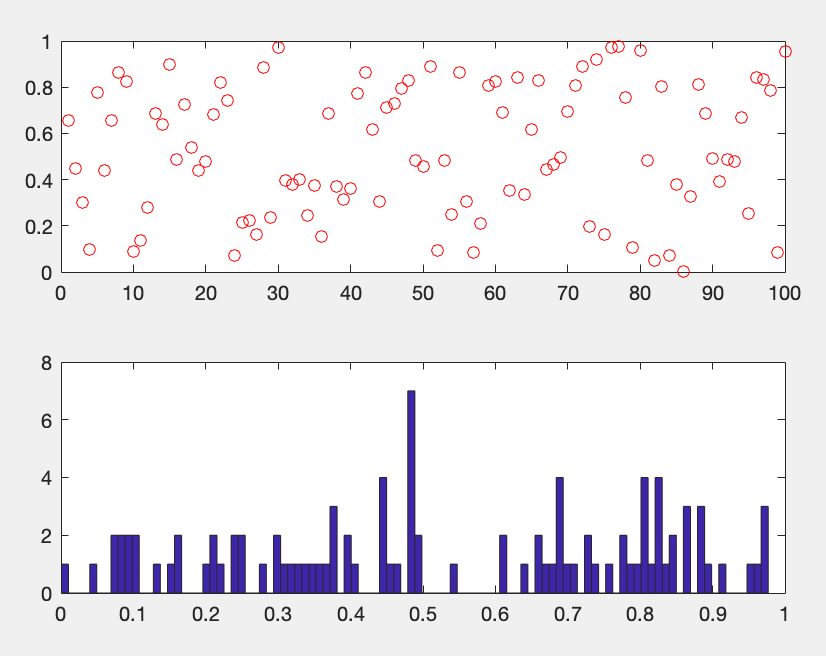
\includegraphics[width=\linewidth]{imgs/q1d_100.png}
        \caption{\( N=10 \)}
    \end{subfigure}
    \hfill
    \begin{subfigure}[h]{0.45\linewidth}
        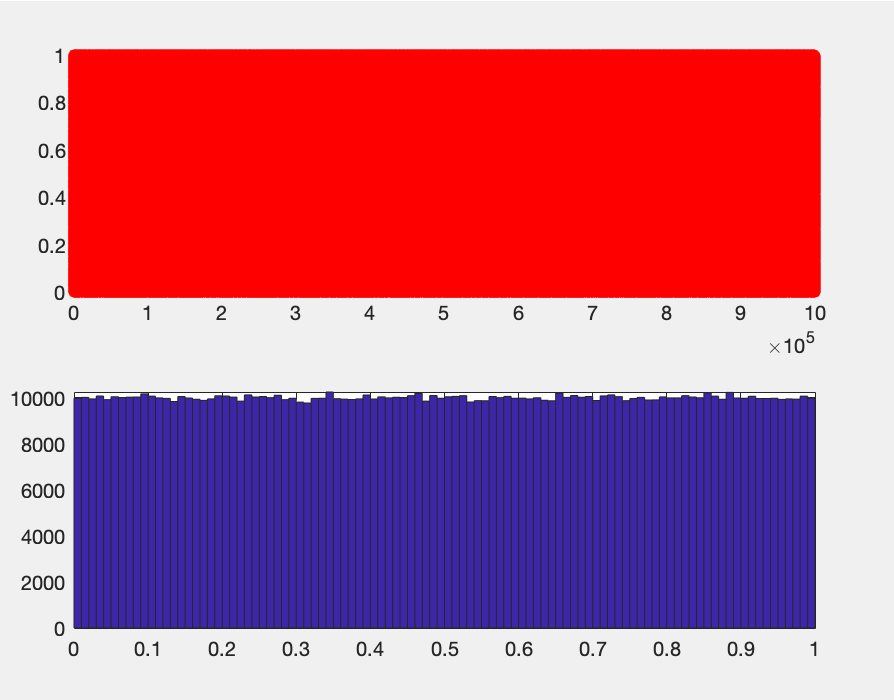
\includegraphics[width=\linewidth]{imgs/q1d_1000000.png}
        \caption{\( N=1000000\)}
    \end{subfigure}
\end{figure}
We can see that as \( \lim_{N\to \infty}\) the distrubution becomes more like a uniform distrubution. 


\newpage
\section{Question 2}
\subsection{(a)}
\begin{figure}[H]
    \begin{subfigure}[h]{0.45\linewidth}
        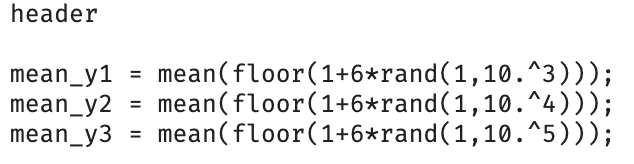
\includegraphics[width=\linewidth]{imgs/q2a_code.png}
        \caption{Code for 2a}
    \end{subfigure}
    \hfill
    \begin{subfigure}[h]{0.45\linewidth}
        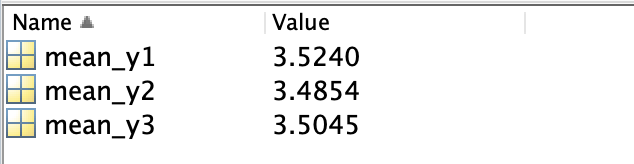
\includegraphics[width=\linewidth]{imgs/q2a_result.png}
        \caption{Results for 2a}
    \end{subfigure}
\end{figure}
Yes as \( N \) increases the resulting average converges to 3.5

\subsection{(b)}

\begin{figure}[H]
    \centering
    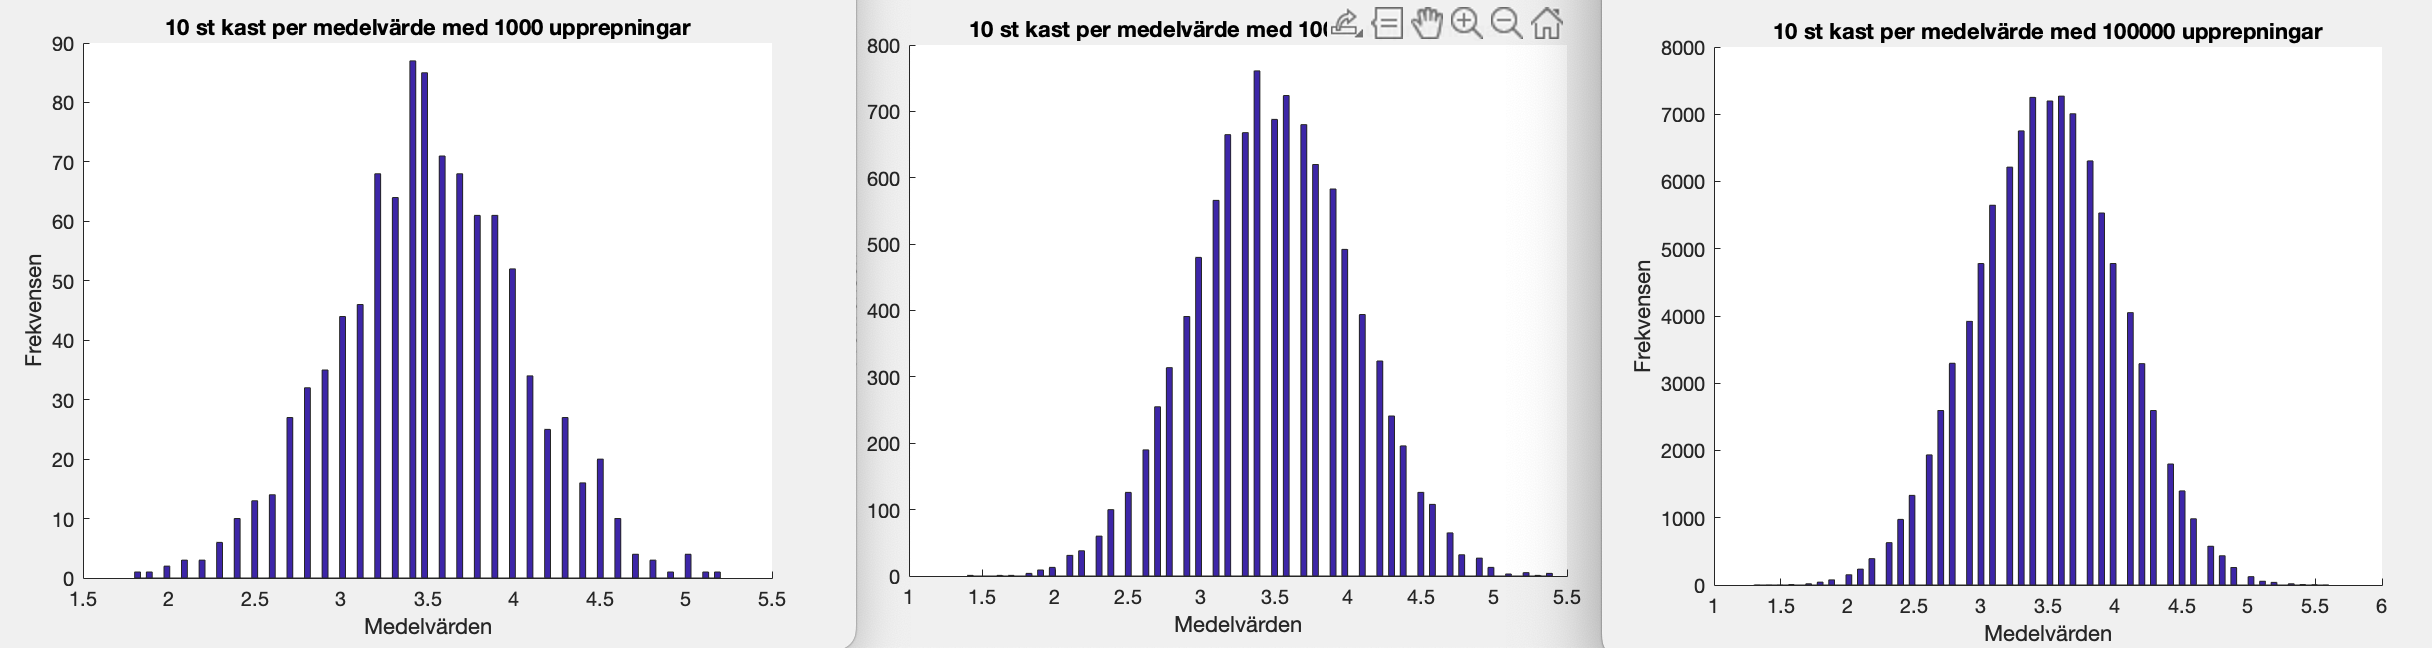
\includegraphics[width=\linewidth]{imgs/q2b.png}
    \caption{Results for 2b}
\end{figure}
We can see that it becomes more like a normal distribution as we repeat the test more times

\newpage
\subsection{(c)}
\begin{figure}[H]
    \centering
    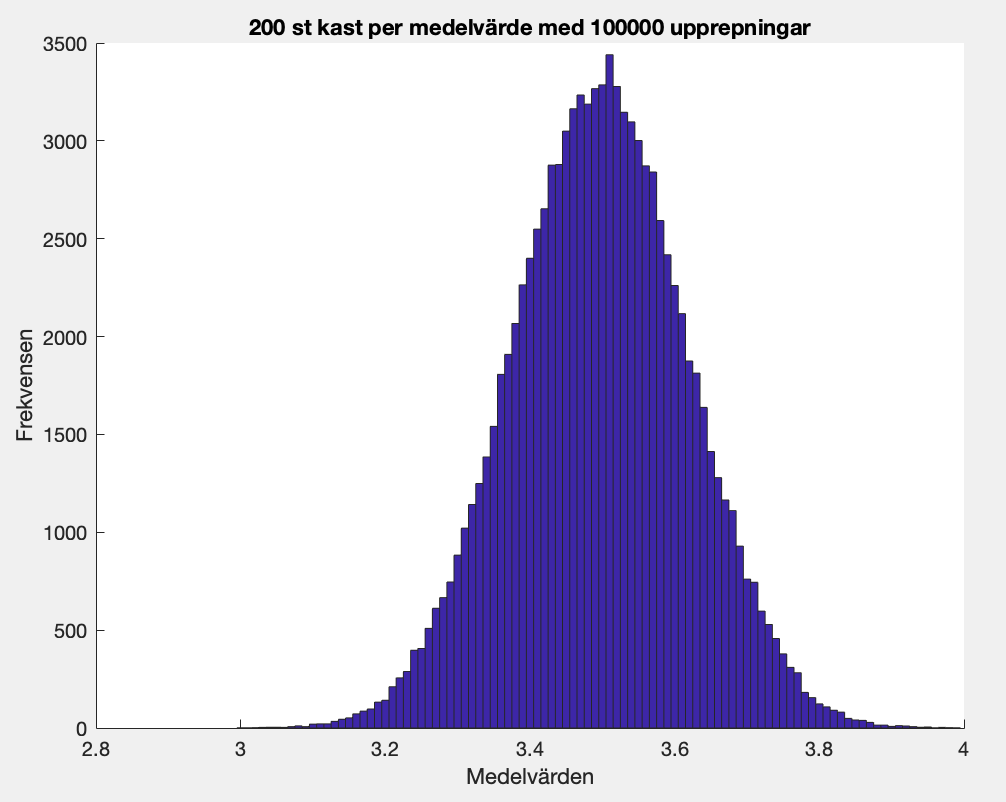
\includegraphics[width=0.5\linewidth]{imgs/q2c_result.png}
    \caption{Results for 2c}
\end{figure}
It's possible to observe that the variance of this result is lower than that of question 2b. This is 
logical since we take the mean of more throws before adding them. This should create fewer outliers and thus lower the variance.

\subsection{(d)}
\begin{figure}[H]
    \begin{subfigure}[h]{0.45\linewidth}
        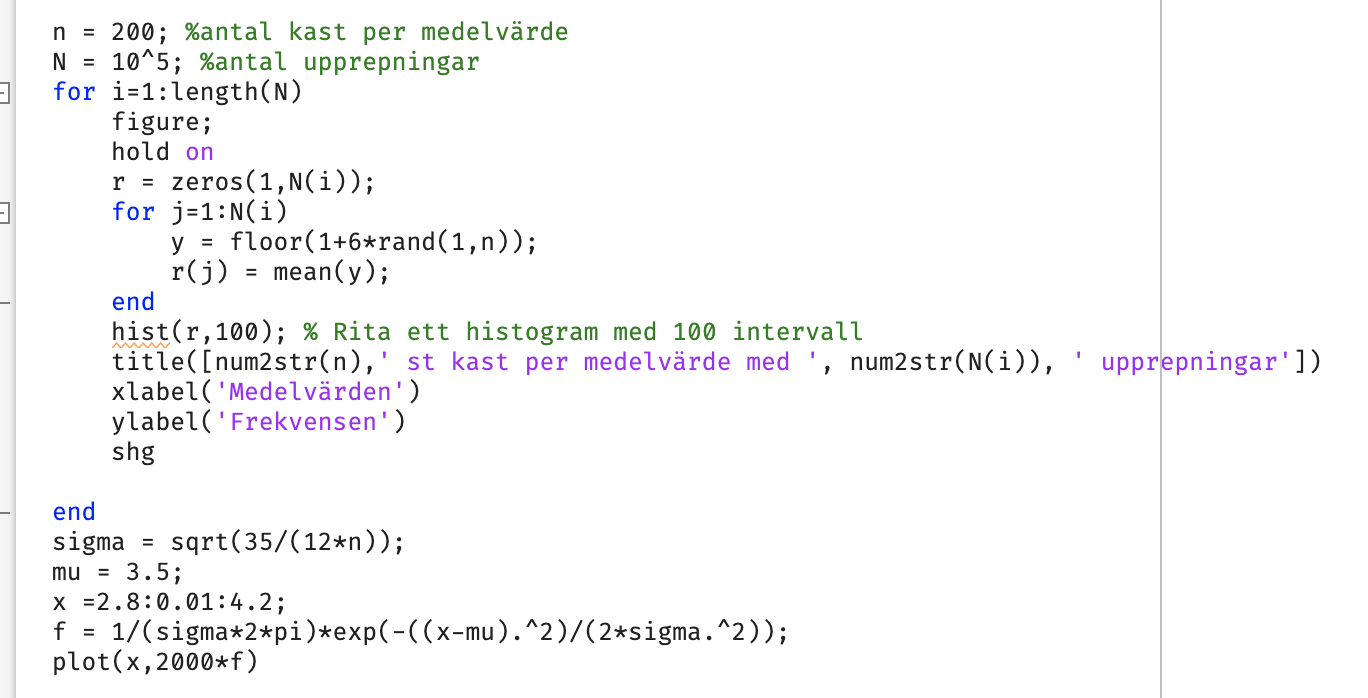
\includegraphics[width=\linewidth]{imgs/q2d_code.png}
        \caption{Code for 2d}
    \end{subfigure}
    \hfill
    \begin{subfigure}[h]{0.45\linewidth}
        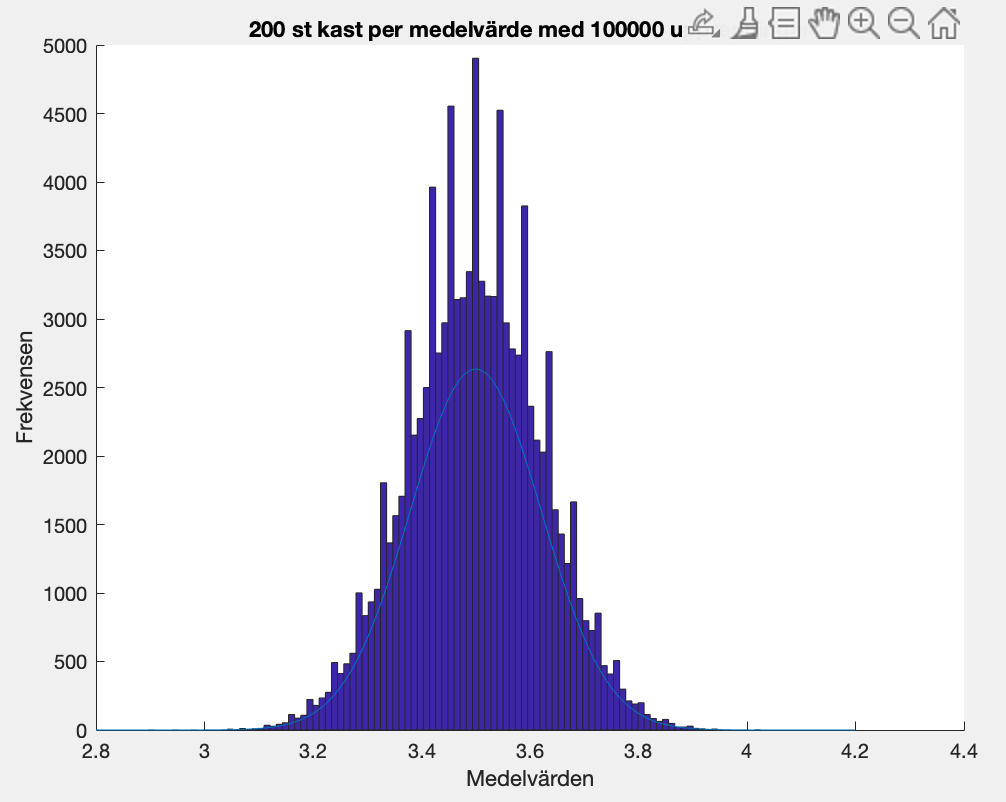
\includegraphics[width=\linewidth]{imgs/q2d_graph.png}
        \caption{Results for 2d}
    \end{subfigure}
\end{figure}
The magnitude of the function \( f \) is dependent on \( n \) so we need to multiply the function 
to make it fit our histogram.

\subsection{(e)}
\begin{figure}[H]
    \begin{subfigure}[h]{0.45\linewidth}
        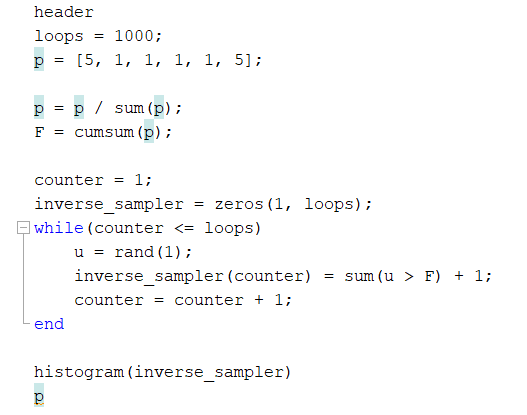
\includegraphics[width=\linewidth]{imgs/q2e_code.png}
        \caption{Code for 2e}
    \end{subfigure}
    \hfill
    \begin{subfigure}[h]{0.45\linewidth}
        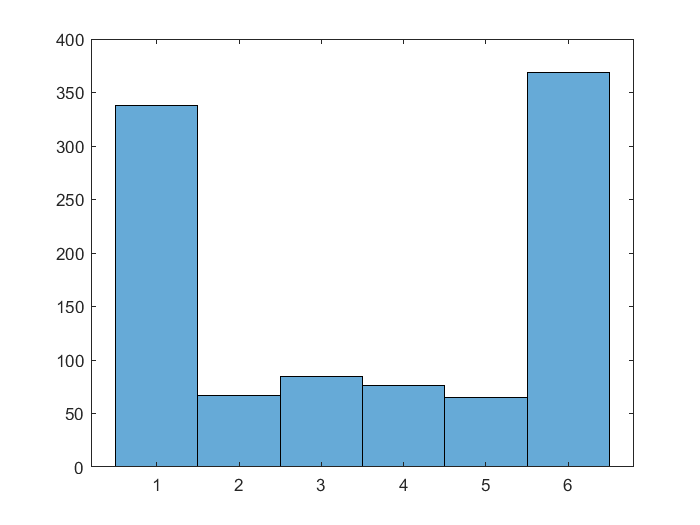
\includegraphics[width=\linewidth]{imgs/q2e_histogram.png}
        \caption{Histogram for 2e}
    \end{subfigure}
\end{figure}
    \begin{figure}[h]
        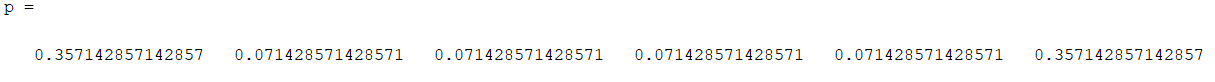
\includegraphics[width=\linewidth]{imgs/q2e_p.png}
        \caption{Probability of p}
    \end{figure}
    \hfill

Comparing the probabilities for the different outcomes of p with the histogram we can see that they match up well. Where p(1) and p(6) is roughly 5 times greater than p(2), p(3), p(4), p(5). 
Looking at their y-values in the histogram they are about a fifth of the height at 1 and 6.

To generate a continuous random variable with a density function, you would take the cumulative sum of the density function and then find the inverse of it. Lastly compute it as \(X = F - 1(u)\).

\newpage
\section{Question 3}

\subsection{(a)}
\begin{figure}[H]
    \begin{subfigure}[h]{0.45\linewidth}
        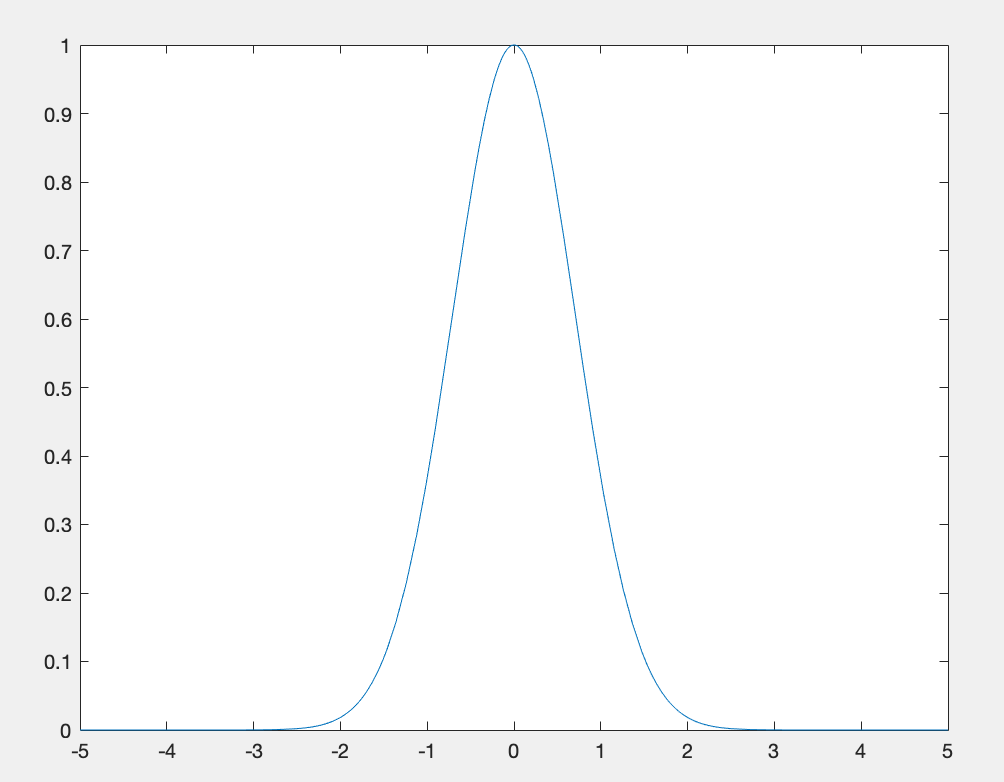
\includegraphics[width=\linewidth]{imgs/q3a_1d_100.png}
        \caption{1D 100}
    \end{subfigure}
    \hfill
    \begin{subfigure}[h]{0.45\linewidth}
        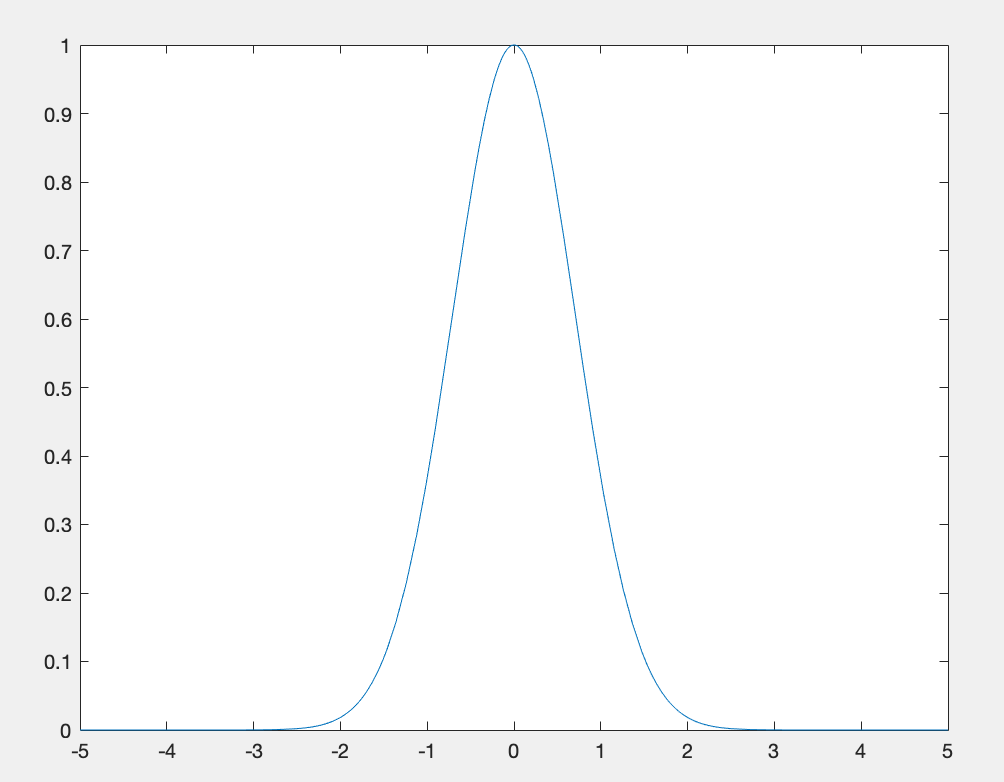
\includegraphics[width=\linewidth]{imgs/q3a_1d_1000000.png}
        \caption{1D 1000000}
    \end{subfigure}
\end{figure}

\begin{figure}[H]
    \begin{subfigure}[h]{0.45\linewidth}
        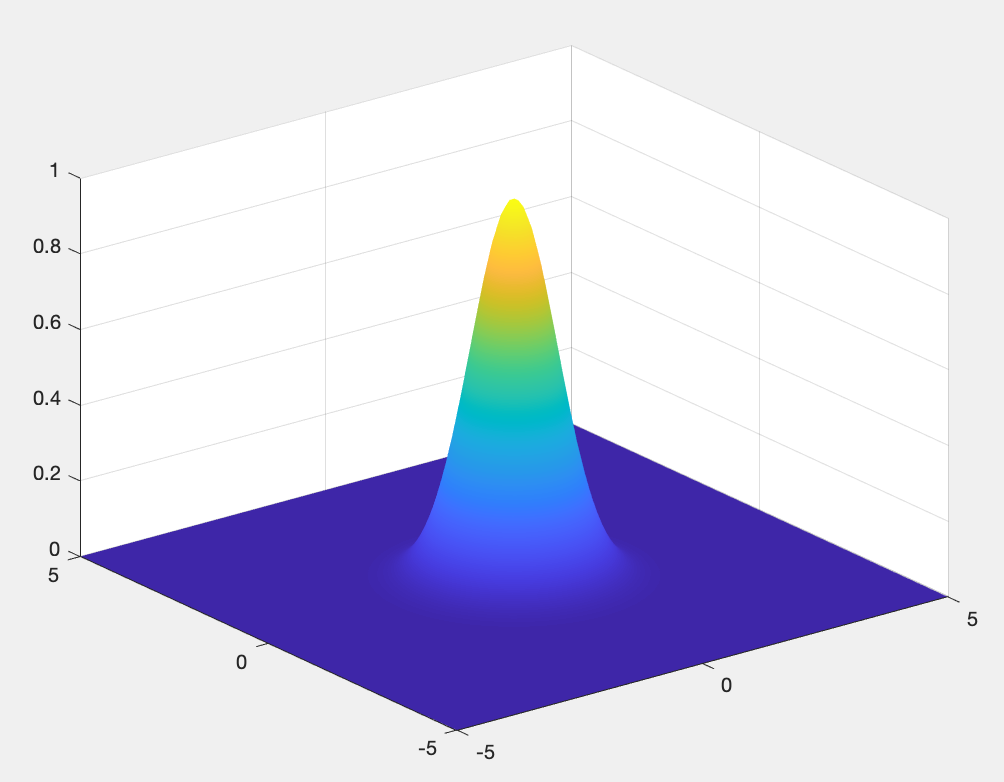
\includegraphics[width=\linewidth]{imgs/q3a_2d_100.png}
        \caption{2D 100}
    \end{subfigure}
    \hfill
    \begin{subfigure}[h]{0.45\linewidth}
        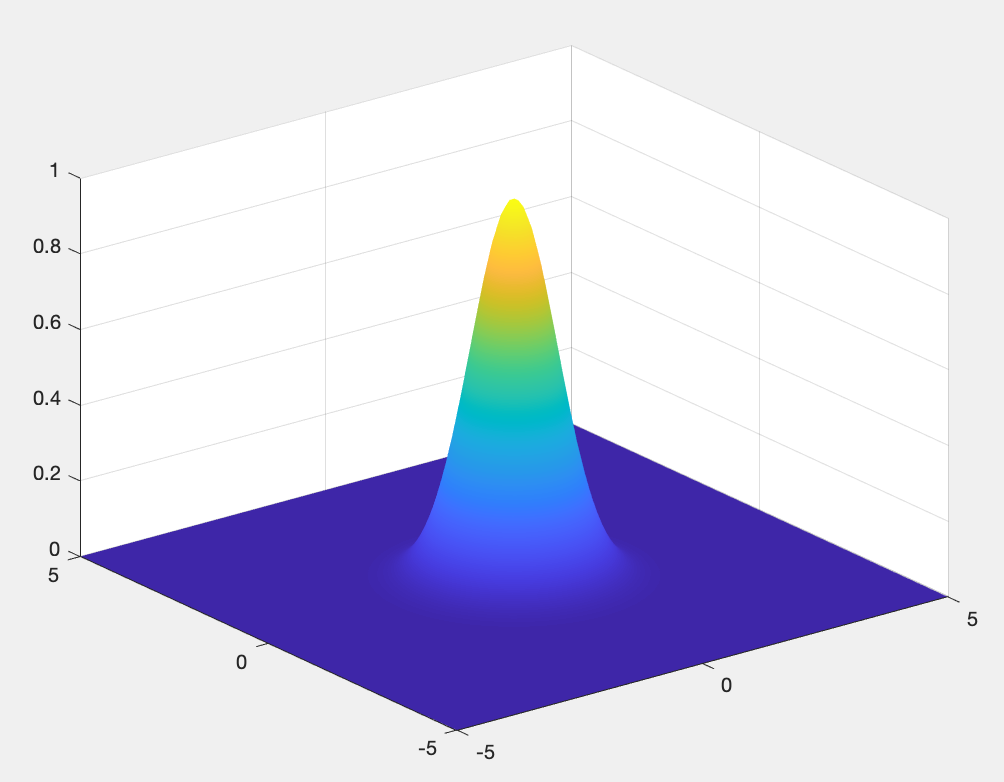
\includegraphics[width=\linewidth]{imgs/q3a_2d_1000000.png}
        \caption{2D 1000000}
    \end{subfigure}
\end{figure}

\begin{figure}
    \centering
    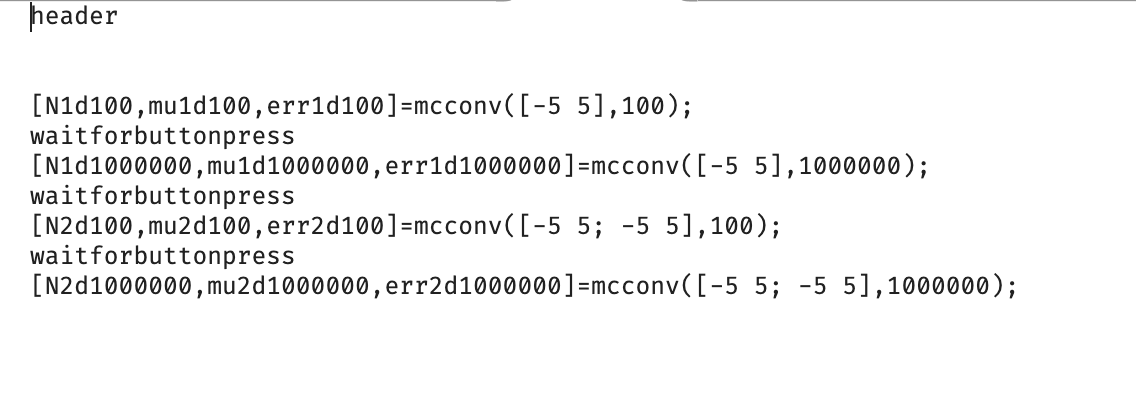
\includegraphics[width=\linewidth]{imgs/q3a_code.png}
    \caption{Code for question 3a}
\end{figure}

\subsection{(b)}

\begin{figure}[H]
    \centering
    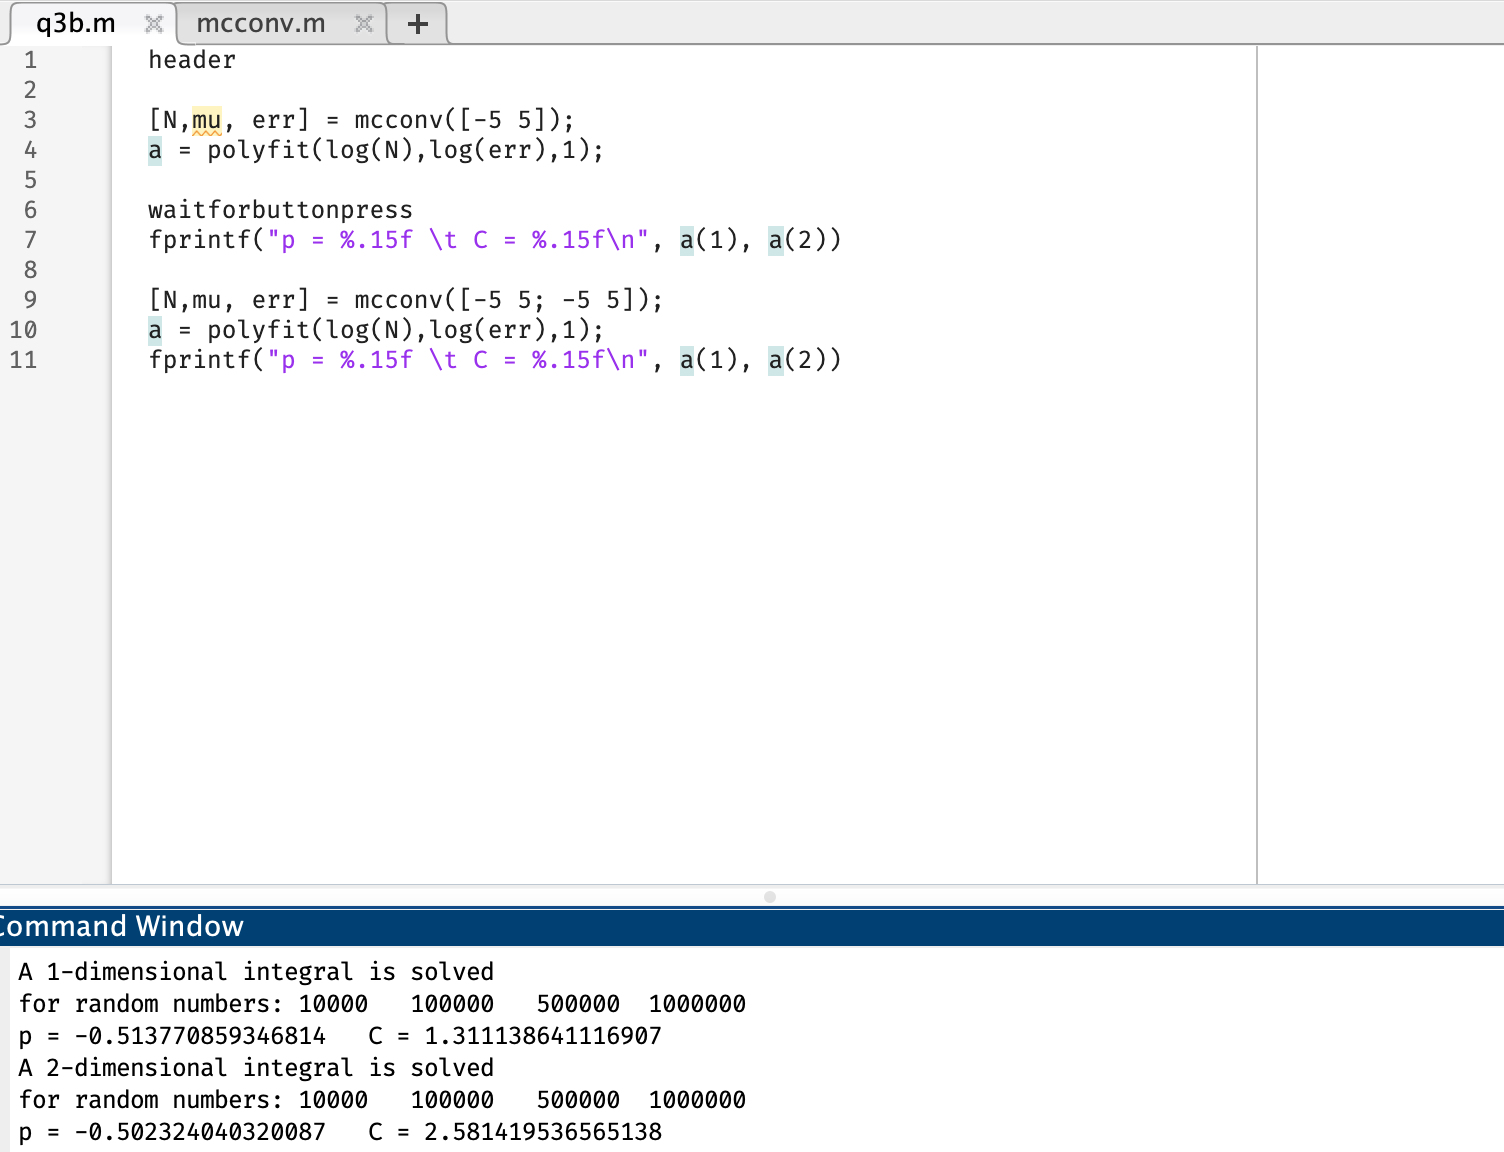
\includegraphics[width=\linewidth]{imgs/q3b.png}
    \caption{Question 3b}
    \label{q3b}
\end{figure}
We can see that \( p \) does not change very much depending on the dimension.
However \( C \) increases a lot when increasing dimention as you can see in Figure \ref{q3b}.

\subsection{(c)}

Monte Carlo is more efficient in higher dimensions than the Trapezoid method. This is because of the \textit{Curse of Dimensionality}
which states that when dimensionality.
\newpage
\section{Question 4}

\begin{figure}[H]
    \centering
    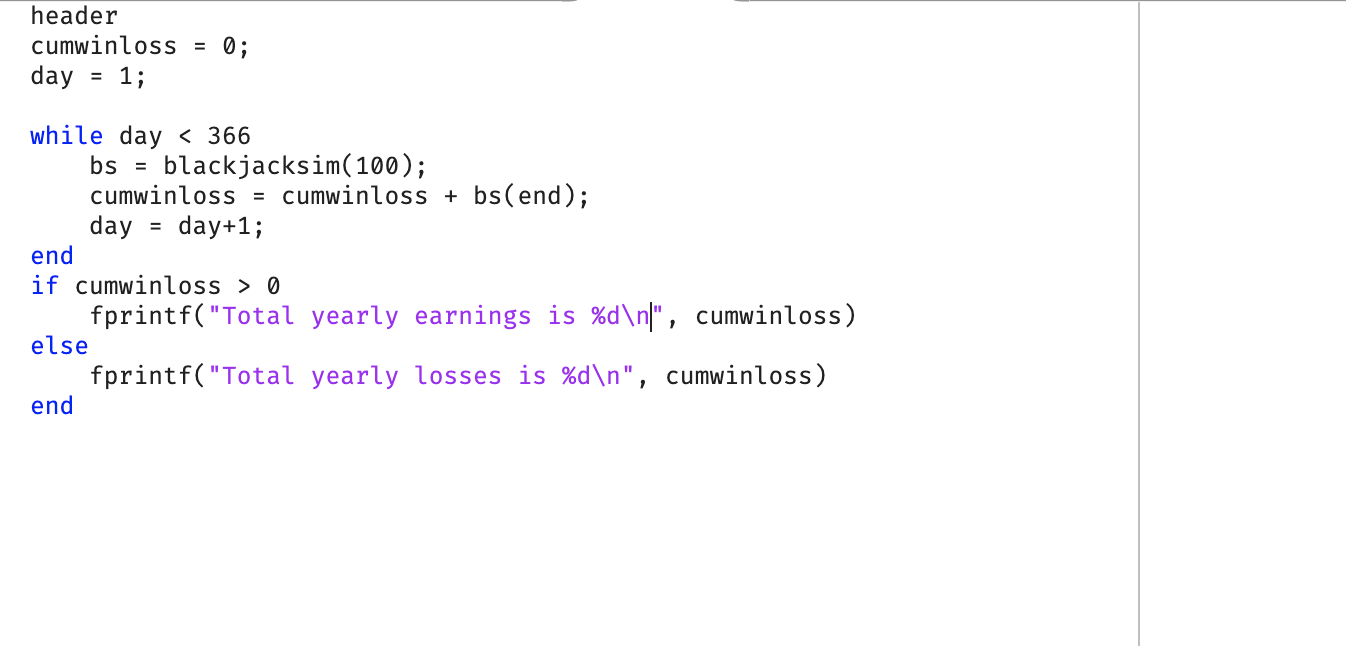
\includegraphics[width=0.8\linewidth]{imgs/q4_code.png}
    \caption{Code for question 4}
\end{figure}

Running this script usually yields a cumulative return of around -8000 to +2000. However it more often than not
ends up being a net loss for the year.



\end{document}
